%-----------------------------------------------------------------------------------------------------------------------------------------------%
%	The MIT License (MIT)
%
%	Copyright (c) 2015 Jan Küster
%
%	Permission is hereby granted, free of charge, to any person obtaining a copy
%	of this software and associated documentation files (the "Software"), to deal
%	in the Software without restriction, including without limitation the rights
%	to use, copy, modify, merge, publish, distribute, sublicense, and/or sell
%	copies of the Software, and to permit persons to whom the Software is
%	furnished to do so, subject to the following conditions:
%	
%	THE SOFTWARE IS PROVIDED "AS IS", WITHOUT WARRANTY OF ANY KIND, EXPRESS OR
%	IMPLIED, INCLUDING BUT NOT LIMITED TO THE WARRANTIES OF MERCHANTABILITY,
%	FITNESS FOR A PARTICULAR PURPOSE AND NONINFRINGEMENT. IN NO EVENT SHALL THE
%	AUTHORS OR COPYRIGHT HOLDERS BE LIABLE FOR ANY CLAIM, DAMAGES OR OTHER
%	LIABILITY, WHETHER IN AN ACTION OF CONTRACT, TORT OR OTHERWISE, ARISING FROM,
%	OUT OF OR IN CONNECTION WITH THE SOFTWARE OR THE USE OR OTHER DEALINGS IN
%	THE SOFTWARE.
%	
%
%-----------------------------------------------------------------------------------------------------------------------------------------------%


%============================================================================%
%
%	DOCUMENT DEFINITION
%
%============================================================================%

%we use article class because we want to fully customize the page and dont use a cv template
\documentclass[10pt,A4]{article}	
\usepackage[colorlinks=true, citecolor=red, urlcolor=blue]{hyperref}

%----------------------------------------------------------------------------------------
%	ENCODING
%----------------------------------------------------------------------------------------

%we use utf8 since we want to build from any machine
\usepackage[utf8]{inputenc}		

%----------------------------------------------------------------------------------------
%	LOGIC
%----------------------------------------------------------------------------------------

% provides \isempty test
\usepackage{xifthen}
\usepackage[notransparent]{svg}
%----------------------------------------------------------------------------------------
%	FONT
%----------------------------------------------------------------------------------------

% some tex-live fonts - choose your own

% \usepackage[defaultsans]{droidsans}
% \usepackage[default]{comfortaa}
% \usepackage{cmbright}
% \usepackage[default]{raleway}
% \usepackage{fetamont}
\usepackage[default]{gillius}
% \usepackage[light,math]{iwona}
% \usepackage[thin]{roboto} 

% set font default
\renewcommand*\familydefault{\sfdefault} 	
\usepackage[T1]{fontenc}

% more font size definitions
\usepackage{moresize}		

\usepackage{fontawesome}

%----------------------------------------------------------------------------------------
%	PAGE LAYOUT  DEFINITIONS
%----------------------------------------------------------------------------------------

%debug page outer frames
%\usepackage{showframe}			


%define page styles using geometry
\usepackage[a4paper]{geometry}		

% for example, change the margins to 2 inches all round
\geometry{top=1cm, bottom=-.6cm, left=0.4cm, right=1cm} 	


%less space between header and content
\setlength{\headheight}{-5pt}		


%customize entries left, center and right
%\lhead{}
%\chead{ \small{Jan Küster  $\cdot$ Consultant and Software Engineer $\cdot$  Bremen, Germany  $\cdot$  \textcolor{sectcol}{\textbf{info@jankuester.com}}  $\cdot$ +49 176 313 *** **}}
%\rhead{}


%indentation is zero
\setlength{\parindent}{0mm}

%----------------------------------------------------------------------------------------
%	TABLE /ARRAY DEFINITIONS
%---------------------------------------------------------------------------------------- 

%for layouting tables
\usepackage{multicol}			
\usepackage{multirow}

%extended aligning of tabular cells
\usepackage{array}

\newcolumntype{x}[1]{%
>{\raggedleft\hspace{0pt}}p{#1}}%


%----------------------------------------------------------------------------------------
%	GRAPHICS DEFINITIONS
%---------------------------------------------------------------------------------------- 

%for header image
\usepackage{graphicx}

%for floating figures
\usepackage{wrapfig}
\usepackage{float}
%\floatstyle{boxed} 
%\restylefloat{figure}

%for drawing graphics		
\usepackage{tikz}				
\usetikzlibrary{shapes, backgrounds,mindmap, trees}


%----------------------------------------------------------------------------------------
%	Color DEFINITIONS
%---------------------------------------------------------------------------------------- 
\usepackage{transparent}
\usepackage{color}

%accent color
\definecolor{complcol}{RGB}{250,150,10}

%dark background color
\definecolor{bgcol}{RGB}{110,110,110}

%light background / accent color
\definecolor{softcol}{RGB}{225,225,225}

\definecolor{sectcol}{RGB}{0,120,150}


%Package for links, must be the last package used
%\usepackage[hidelinks]{hyperref}

%============================================================================%
%
%
%	DEFINITIONS
%
%
%============================================================================%

% returns minipage width minus two times \fboxsep
% to keep padding included in width calculations
\newcommand{\mpwidth}{\linewidth-\fboxsep-\fboxsep}
	

%----------------------------------------------------------------------------------------
% 	ARROW GRAPHICS in Tikz
%----------------------------------------------------------------------------------------

% a six pointed arrow poiting to the left
\newcommand{\tzlarrow}{(0,0) -- (0.2,0) -- (0.3,0.2) -- (0.2,0.4) -- (0,0.4) -- (0.1,0.2) -- cycle;}	

% include the left arrow into a tikz picture
% param1: fill color
%
\newcommand{\larrow}[1]
{\begin{tikzpicture}[scale=0.58]
	 \filldraw[fill=#1!100,draw=#1!100!black]  \tzlarrow
 \end{tikzpicture}
}

% a six pointed arrow poiting to the right
\newcommand{\tzrarrow}{ (0,0.2) -- (0.1,0) -- (0.3,0) -- (0.2,0.2) -- (0.3,0.4) -- (0.1,0.4) -- cycle;}

% include the right arrow into a tikz picture
% param1: fill color
%
\newcommand{\rarrow}
{
\begin{tikzpicture}[scale=0.7]
	\filldraw[fill=sectcol!100,draw=sectcol!100!black] \tzrarrow
 \end{tikzpicture}
}

%----------------------------------------------------------------------------------------
%	custom sections
%----------------------------------------------------------------------------------------

% create a coloured box with arrow and title as cv section headline
% param 1: section title
%
\newcommand{\cvsection}[1]
{
\colorbox{sectcol}{\mystrut \makebox[1\mpwidth][l]{
\larrow{bgcol} \hspace{-8pt} \larrow{bgcol} \hspace{-8pt} \larrow{bgcol} \textbf{\textcolor{white}{\uppercase{#1}}}\hspace{4pt}
}}\\
}

% create a coloured arrow with title as cv meta section section
% param 1: meta section title
%
\newenvironment{metasection}[1] {
	\vspace{6pt}
	\begin{center}
		\textcolor{white}{\large{\uppercase{#1}}}\\
	\normalsize
	\parbox{0.7\mpwidth}{\textcolor{white}	\hrule}
}{\end{center}}

%----------------------------------------------------------------------------------------
%	 CV EVENT
%----------------------------------------------------------------------------------------

% creates a stretched box as cv entry headline followed by some paragraphs about 
% the work you did
% param 1:	event time i.e. 2014 or 2011-2014 etc.
% param 2:	event name (what did you do?)
% param 3:	institution (where did you work / study)
% param 4:	list of paragraphs outlining your contributions, see example usage below
%
\newcommand{\cvevent}[4]
{
\vspace{6pt}
	\begin{tabular*}{1\mpwidth}{p{0.55\mpwidth}  x{0.42\mpwidth}}
 	\textcolor{black}{\textbf{#2}} & \textcolor{complcol}{#3}, \textcolor{bgcol}{#1} 
	\end{tabular*}
\vspace{0pt}
\textcolor{softcol}{\hrule}
\vspace{6pt}
	\cvlist {#4}
\vspace{-6pt}
}

% formats a list of strings with variable length for use in `\cvevent`
% param 1: a list of strings outlining your contributions
\newcommand{\cvlist}[1] {
    \foreach \listitem in {#1}
    {
        \begin{tabular*}
            {1\mpwidth}{p{1.2\mpwidth}}
            \parbox{1\mpwidth}{\larrow{softcol} \listitem}
            \vspace{3pt}
        \end{tabular*}
    }
}

% creates a stretched box as 
\newcommand{\cveventmeta}[2]
{
	\mbox{\mystrut \hspace{87pt}\textit{#1}}\\
	#2
}

%----------------------------------------------------------------------------------------
% CUSTOM STRUT FOR EMPTY BOXES
%----------------------------------------- -----------------------------------------------
\newcommand{\mystrut}{\rule[-.3\baselineskip]{0pt}{\baselineskip}}

%----------------------------------------------------------------------------------------
% CUSTOM LOREM IPSUM
%----------------------------------------------------------------------------------------
\newcommand{\lorem}
{Lorem ipsum dolor sit amet, consectetur adipiscing elit. Donec a diam lectus.}


% use to vertically center content
% credits to: http://tex.stackexchange.com/questions/7219/how-to-vertically-center-two-images-next-to-each-other
\newcommand{\vcenteredinclude}[1]{\begingroup
\setbox0=\hbox{\includegraphics{#1}}%
\parbox{\wd0}{\box0}\endgroup}

% use to vertically center content
% credits to: http://tex.stackexchange.com/questions/7219/how-to-vertically-center-two-images-next-to-each-other
\newcommand*{\vcenteredhbox}[1]{\begingroup
\setbox0=\hbox{#1}\parbox{\wd0}{\box0}\endgroup}

%----------------------------------------------------------------------------------------
%	ICON-SET EMBEDDING
%---------------------------------------------------------------------------------------- 

% at this point we simplify our icon-embedding by simply referring to a set of png images.
% if you find a good way of including svg without conflicting with other packages you can
% replace this part
\newcommand{\icon}[3]{\makebox(#2, #2){\textcolor{#3}{\csname fa#1\endcsname}}}	%icon shortcut
\newcommand{\icontext}[4]{ 						%icon with text shortcut
	\vcenteredhbox{\icon{#1}{#2}{#4}} \vcenteredhbox{\textcolor{#4}{#3}}
}
\newcommand{\iconhref}[5]{ 						%icon with website url
    \vcenteredhbox{\icon{#1}{#2}{#5}} \href{#4}{\textcolor{#5}{#3}}
}

\newcommand{\iconemail}[5]{ 						%icon with email link
    \vcenteredhbox{\icon{#1}{#2}{#5}} \href{mailto:#4}{\textcolor{#5}{#3}}
}



%============================================================================%
%
%
%
%	DOCUMENT CONTENT
%
%
%
%============================================================================%
\begin{document}
\fcolorbox{white}{white}{\begin{minipage}[c][0.95\textheight][t]{0.69\linewidth}


%---------------------------------------------------------------------------------------
%	TITLE HEADLINE
%----------------------------------------------------------------------------------------
\vspace{-3pt}
% use this for multiple words like working titles etc.
%\hspace{-0.25\linewidth}\colorbox{bgcol}{\makebox[1.5\linewidth][c]{\hspace{46pt}\HUGE{\textcolor{white}{\uppercase{M.Sc. Jan Küster}} } \textcolor{sectcol}{\rule[-1mm]{1mm}{0.9cm}} \parbox[b]{5cm}{   \large{ \textcolor{white}{{IT Consultant}}}\\
% \large{ \textcolor{white}{{JS Fullstack Engineer}}}}
%}}

% use this for single words, e.g. CV or RESUME etc.
\colorbox{bgcol}{\makebox[\mpwidth][c]{\HUGE{\textcolor{white}{\uppercase{Marouane Zellou}} } \textcolor{sectcol}{\rule[-1mm]{1mm}{0.9cm}} \HUGE{\textcolor{white}{\uppercase{CV}} } }}

%----------------------------------------------------------------------------------------
%	HEADER IMAGE
%----------------------------------------------------------------------------------------


%\hspace{-1.6cm}
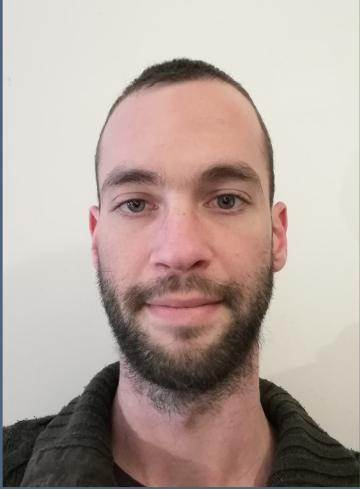
\includegraphics[width=0.3\mpwidth]{photomoi.jpg}	%trimming relative to image size

%---------------------------------------------------------------------------------------
%	SUMMARY
%----------------------------------------------------------------------------------------
\transparent{0.85}%
\vspace{-120pt}
\hspace{0.4\linewidth}
\colorbox{bgcol}{
	\parbox{0.5\linewidth}{
		\transparent{1}%
		\begin{center}
			\larrow{sectcol}\larrow{sectcol}\textcolor{white}{Proactif, autonome et rigoureux, je suis passionné d’informatique et ai goût prononcé pour le traitement de données. Mon parcours m ’a donné les compétences nécessaires pour mener à bien les projets informatiques répondants aux enjeux contemporains : cloud, infrastructures, IA, data-science}
		\end{center}
	}
}
\vspace{20pt}

%============================================================================%
%
%	CV SECTIONS AND EVENTS (MAIN CONTENT)
%
%============================================================================%

%---------------------------------------------------------------------------------------
%	STATUS
%----------------------------------------------------------------------------------------
\cvsection{Status}

Ingénieur en informatique spécialisé en infrastructure de data science.

\vspace{12pt}

%---------------------------------------------------------------------------------------
%	EXPERIENCE
%----------------------------------------------------------------------------------------
\cvsection{Experience}

%
\cvevent{2021}{Ingénieur recherche et développements}{IGN - Paris}{Calcul haute performance, Stockage S3, Métriques des infrastructures, Détection d'objets et ségmentation sémantique par IA, Web sémantique}

%\textcolor{softcol}{\hrule}


%\cvevent{2014 - 2016}{IT Consultant for IBM XPages and Notes Domino}{We4IT GmbH Bremen}{Realize projects in XPages and We4IT Aveedo, monitor project status, conduct reports}{Integrated Camunda BPMN engine and BPMN.IO modeler in We4IT Aveedo}


%\textcolor{softcol}{\hrule}

%
\cvevent{2020}{Développeur web, BD}{\href{https://www.chu-tours.fr/wp-content/uploads/2020/05/CdP-2020-Recherche_etudeTours_CoCliCo-140520.pdf}{CHRU de Tours}}{Application Vue.js permettant la récolte des informations relatives aux antécédents \newline médicaux et aux symptômes des patients atteints de la Covid-19.}


%\textcolor{softcol}{\hrule}
\vspace{6pt}
\cvevent{2020 - 2018}{Chef de projets informatiques}{MTE - Paris}{Responsable de la collecte{,} du contrôle de la qualité et des redressements des données \newline du logements social en France \href{http://www.statistiques.developpement-durable.gouv.fr/le-parc-locatif-social-au-1er-janvier-2020-0?rubrique=52&dossier=1049}{RPLS}, Développement d’applications R (\href{http://dataviz.statistiques.developpement-durable.gouv.fr/RPLS/}{Shiny}) facilitant l’accès aux données, Développement d’un \href{https://rdes_dreal.gitlab.io/propre.rpls/index.html}{paquet R} de production de rapports automatisés}


%\textcolor{softcol}{\hrule}


%

\vspace{6pt}
%---------------------------------------------------------------------------------------
%	EDUCATION SECTION
%--------------------------------------------------------------------------------------
\cvsection{Parcours académique}

\cvevent{2018}{Diplôme d’ingénieur des travaux publics de l’Etat}{ENTPE}{Master mobilité dans les mega-cites {(}Université de Lyon 1{)}}
\vspace{6pt}

\cvevent{2018}{Stage de fin d'études}{LICIT, ENTPE Lyon}{Etude de l’intégration de la dynamique du trafic dans la résolution des algorithmes de \newline plus court chemin, Article présenté au TRB : \newline \href{https://nicolaschiabaut.weebly.com/publications.html}{Toward a Traffic-Dependent Optimization of Urban Freight Deliveries \newline  Building a Benchmark Dataset and Analyzing Effects of Traffic Flow Dynamics}}
\vspace{6pt}

% \textcolor{softcol}{\hrule}

\cvevent{2017}{Stage de recherche}{UTRC, City College of New York}{Etude de performance des algorithmes de plus courts chemin dépendants du trafic, Article publié au Transportation Research Borad et présenté à la l'International \newline Federation of Operational Research Societies : \newline  \href{https://journals.sagepub.com/doi/abs/10.1177/0361198118797829}{Probabilistic Fleet Sizing and Routing Problem to Minimize Mobility Disparities}}

%

%\textcolor{softcol}{\hrule}

%

%\textcolor{softcol}{\hrule}

%


\end{minipage}}%
\fcolorbox{white}{sectcol}{\begin{minipage}[c][0.95\textheight][t]{0.28\linewidth}


\begin{metasection}{Contact}

	\icontext{MapMarker}{12}{Paris, Franjce}{white}\\[6pt]
    \icontext{MobilePhone}{12}{+33 6 66 03 44 14}{white}\\[6pt]
    \iconemail{Send}{12}{mzellou@protonmail.com}{mzellou@protonmail.com}{white}\\[6pt]
    \iconhref{Github}{12}{https://github.com/MZellou}{https://github.com/MZellou}{white}\\[6pt]

\end{metasection}

%----------------------------------------------------------------------------------------
%	META SECTION
%----------------------------------------------------------------------------------------




\begin{metasection}{Technologies}

\textcolor{white}{
	\icontext{Code}{12}{Python-R}{white} \\[6pt]
	\icontext{Code}{12}{JS-HTML-CSS}{white} \\[6pt]
	\icontext{Code}{12}{Docker}{white} \\[6pt]
	\icontext{Code}{12}{Bash}{white} \\[6pt]
	\icontext{Database}{12}{POSTGRES}{white} \\[6pt]
	\icontext{Github}{12}{Git}{white} \\[6pt]
	\icontext{MapMarker}{12}{SIG}{white} \\[6pt]
	%\includesvg[width=1.5cm,height=1.5cm]{docker}
	}
\end{metasection}

\begin{metasection}{Outils}

\textcolor{white}{
	\icontext{CodeFork}{12}{Portainer}{white}\\[6pt] 
	\icontext{Dashboard}{12}{Grafana-Prometheus}{white} \\[6pt]
	\icontext{Cloud}{12}{AWS S3-Minio}{white}  \\[6pt] 
	\icontext{MapMarker}{12}{Leaflet-Geoserver}{white} \\[6pt] 
	\icontext{ObjectUngroup}{12}{Pytorch-Yolo}{white} \\[6pt]
	%\icontext{Leaf}{12}{}{white}
}
\end{metasection}

\begin{metasection}{Compétences à développer}

	\icontext{Code}{12}{Réseau}{white}\\
	\icon{Star}{12}{complcol}\icon{Star}{12}{complcol}\icon{Star}{12}{complcol}\icon{Star}{12}{complcol}\icon{Star}{12}{complcol}\icon{Star}{12}{complcol}\icon{Star}{12}{complcol}\icon{Star}{12}{complcol}\icon{Star}{12}{white}\icon{Star}{12}{white}\\[6pt]
	
	\icontext{CommentsO}{12}{Infrastructures}{white}\\
	\icon{Star}{12}{complcol}\icon{Star}{12}{complcol}\icon{Star}{12}{complcol}\icon{Star}{12}{complcol}\icon{Star}{12}{complcol}\icon{Star}{12}{complcol}\icon{Star}{12}{white}\icon{Star}{12}{white}\icon{Star}{12}{white}\icon{Star}{12}{white}\\[6pt]
	
	\icontext{Lock}{12}{SSI}{white}\\
	\icon{Star}{12}{complcol}\icon{Star}{12}{complcol}\icon{Star}{12}{complcol}\icon{Star}{12}{complcol}\icon{Star}{12}{complcol}\icon{Star}{12}{complcol}\icon{Star}{12}{white}\icon{Star}{12}{white}\icon{Star}{12}{white}\icon{Star}{12}{white}\\[6pt]
\end{metasection}	

\begin{metasection}{Loisirs}

\textcolor{white}{\LARGE{\icon{Gamepad}{24}{white} \icon{Headphones}{24}{white}  \icon{Plane}{24}{white}}}  \\[6pt]
\textcolor{white}{\LARGE{\icon{Anchor}{24}{white} \icon{CommentingO}{24}{white}  \icon{Compass}{24}{white}}}
\end{metasection}

\begin{metasection}{Systèmes d'exploitation}

\textcolor{white}{\LARGE{\icon{Linux}{24}{white} \icon{Apple}{24}{white}  \icon{Windows}{24}{white}}}

\end{metasection}

%---------------------------------------------------------------------------------------
%	QR CODE (optional)
%----------------------------------------------------------------------------------------

% \vspace{12pt}
% \begin{center}
% \includegraphics[width=0.35\mpwidth]{qrcode}
% \end{center}

\end{minipage}}

%-------------------------------------------------------------------------------------------------
%	ARTIFICIAL FOOTER (fancy footer cannot exceed linewidth) 
%--------------------------------------------------------------------------------------------------

\null
\vspace*{\fill}
\hspace{-0.25\linewidth}\colorbox{bgcol}{\makebox[1.5\linewidth][c]{\mystrut \small \textcolor{white}{}}}\\[-6pt]

%============================================================================%
%
%
%
%	DOCUMENT END
%
%
%
%============================================================================%
\end{document}